\chapter{Dedicibilità}
In questo capitolo iniziamo ad investigare la potenza degli algoritmi nella risoluzione di problemi. Dimostreremo che alcuni problemi possono essere risolti in maniera algoritmica ed altri no. Il nostro obiettivo è esplorare i limiti della risolvibilità algoritmica dei problemi.

\section{Linguaggi decidibili}
In questa sezione diamo alcuni esempi di linguaggi che sono decidibili mediante algoritmi.

\subsection{Problemi decidibili relativi a linguaggi regolari}
Iniziamo con alcuni problemi computazionali relativi ad automi finiti. 

Ad esempio, il problema dell'accettazione per DFA consiste nel testare se un particolare automa finito deterministico accetta una data stringa, può essere espresso come un linguaggio, $A_{DFA}$. Questo linguaggio contiene le codifiche di tutti i DFA con le stringhe che essi accettano. Definiamo
\begin{equation*}
A_{DFA}=\{\langle B, w\rangle | B \textit{ è un DFA che accetta la stringa di input }w\}
\end{equation*}
Il problema di verificare se un DFA $B$ accetta l'input $w$ coincide con il problema di verificare se $\langle B, w\rangle $ è un elemento del linguaggio $A_{DFA}$. Mostrare che il linguaggio è decidibile equivale a mostrare che il problema computazionale è decidibile.

\begin{Thm}{$A_{DFA}$ è un linguaggio decidibile}{}\label{thm:adfa-decidibile}
\textit{$A_{DFA}$ è un linguaggio decidibile.}

\begin{osservation}
Abbiamo semplicemente bisogno di presentare una TM $M$ che decide $A_{DFA}$.

$M =$ "Su input $\langle B, w\rangle $, dove $B$ è un DFA e $w$ è una stringa:
\begin{enumerate}
    \item Simula $B$ su input $w$.
    \item Se la simulazione termina in uno stato di accettazione, accetta. Se non termina in uno stato di accettazione, rifiuta."
\end{enumerate}    
\end{osservation}

\begin{demonstration}
In primo luogo, esaminiamo l'input $\langle B, w\rangle $. Si tratta di una rappresentazione di un DFA $B$ insieme ad una stringa $w$. Una rappresentazione ragionevole di $B$ è semplicemente una lista delle sue cinque componenti: $Q$, $\Sigma$, $\delta$, $q_0$, ed $F$. Quando $M$ riceve il suo input, per prima cosa verifica se esso rappresenta correttamente un DFA $B$ ed una stringa $w$. In caso contrario, $M$ rifiuta. Poi $M$ effettua direttamente la simulazione. Tiene traccia dello stato corrente di $B$ e della posizione corrente di $B$ nell'input $w$ scrivendo queste informazioni sul suo nastro. Inizialmente, lo stato corrente di $B$ è $q_0$ e la posizione corrente dell'input di $B$ è il simbolo più a sinistra di $w$. Gli stati e le posizioni vengono aggiornati in base alla funzione di transizione specificata $\delta$. Quando $M$ termina l'elaborazione dell'ultimo simbolo di $w$, $M$ accetta l'input se $B$ è in uno stato di accettazione; $M$ rifiuta l'input se $B$ non è in uno stato di accettazione.
\end{demonstration}
\end{Thm}

Possiamo dimostrare un teorema simile per automi a stati finiti non deterministici. Dato
\begin{equation*}
A_{NFA} = \{\langle B,w\rangle  | B \textit{ è un NFA che accetta la stringa di input }w\}
\end{equation*}

\begin{Thm}{$A_{NFA}$ è un linguaggio decidibile}{}\label{thm:anfa-decidibile}
\textit{$A_{NFA}$ è un linguaggio decidibile.}

\begin{demonstration}
Presentiamo una TM $N$ che decide $A_{NFA}$. Potremmo progettare $N$ in modo che operi come $M$, simulando un NFA invece di un DFA. Invece, procederemo in modo diverso per illustrare una nuova idea: $N$ usa $M$ come una sottoprocedura. Poichè $M$ è progettata per funzionare con un DFA, $N$ prima converte l'NFA che riceve come input in un DFA e poi lo passa ad $M$.
\end{demonstration}    
\end{Thm}

In modo analogo, possiamo determinare se un'espressione regolare genera una data stringa
\begin{equation*}
A_{REX} = \{\langle R, w\rangle | R\textit{ è un'espressione regolare che genera la stringa }w\}
\end{equation*}

\begin{Thm}{$A_{REX}$ è un linguaggio decidibile}{}\label{thm:arex-decidibile}
\textit{$A_{REX}$ è un linguaggio decidibile.}

\begin{demonstration}
La seguente TM $P$ decide $A_{REX}$.

$P=$ "Su input $\langle R, w\rangle $, dove $R$ è un'espressione regolare e $w$ è una stringa: 
\begin{enumerate}
    \item Converte l'espressione regolare $R$ in un NFA $A$ equivalente, mediante la procedura di conversione.
    \item Esegue la TM $N$ su input $\langle A, w\rangle $.
    \item Se $N$ accetta, accetta; se $N$ rifiuta, rifiuta."
\end{enumerate}
\end{demonstration}
\end{Thm}

I Teoremi \ref{thm:adfa-decidibile}, \ref{thm:anfa-decidibile} e \ref{thm:arex-decidibile} ci dicono che, ai fini della decidibilità, è equivalente presentare alla macchina di Turing un DFA, un NFA, oppure un'espressione regolare, perché la macchina è in grado di convertire una codifica nell'altra.

Ora affrontiamo un diverso tipo di problema concernente gli automi a stati finiti: il test del vuoto per il linguaggio di un automa finito. Dobbiamo determinare se un automa finito accetta una qualche stringa. Consideriamo
\begin{equation*}
E_{DFA}=\{\langle A\rangle| A\textit{ è un DFA e }L(A) = \emptyset\}
\end{equation*}

\begin{Thm}{$E_{DFA}$ è un linguaggio decidibile}{}\label{thm:edfa-decidibile}
\textit{$E_{DFA}$ è un linguaggio decidibile.}

\begin{demonstration}
Il DFA accetta almeno una stringa se e solo se dallo stato iniziale può raggiungere uno stato di accettazione percorrendo il verso delle frecce del DFA. Per verificare questa condizione possiamo progettare una TM $T$ che utilizza un algoritmo di marcatura.

$T =$ "Su input $\langle A\rangle$, dove $A$ è un DFA:    
\begin{enumerate}
    \item Marca lo stato iniziale di $A$.
    \item Ripete fino a quando non vengono più marcati nuovi stati: marca qualsiasi stato che ha una transizione proveniente da uno stato già marcato.
    \item Se nessuno stato di accettazione risulta marcato, accetta; altrimenti, rifiuta."    
\end{enumerate}
\end{demonstration}
\end{Thm}

Il prossimo teorema afferma che determinare se due DFA riconoscono lo stesso linguaggio è decidibile. Sia
\begin{equation*}
EQ_{DFA} =\{\langle A,B \rangle | A\textit{ e }B\textit{ sono DFA e }L(A) = L(B)\}    
\end{equation*}

\begin{Thm}{$EQ_{DFA}$ è un linguaggio decidibile}{}
\textit{$EQ_{DFA}$ è un linguaggio decidibile.}

\begin{demonstration}
Per dimostrare questo teorema usiamo il Teorema \ref{thm:edfa-decidibile}. Costruiamo un nuovo DFA $C$ a partire da $A$ e $B$, dove $C$ accetta solo quelle stringhe che sono accettate da $A$ o da $B$, ma non da entrambi. In particolare, se $A$ e $B$ riconoscono lo stesso linguaggio, $C$ non accetterà nulla. Il linguaggio di C è
\begin{equation*}
L(C) =(L(A) \cap \overline{L(B)}) \cup( \overline{L(A)} \cap L(B))    
\end{equation*}

Questa espressione è a volte denotata come differenza simmetrica di $L(A)$ e $L(B)$. Qui $\overline{L(A)}$ denota il complemento di $L(A)$. La differenza simmetrica è utile perché $L(C) = \emptyset$ se e solo se $L(A) = L(B)$. Una volta che abbiamo costruito $C$ possiamo usare il Teorema \ref{thm:edfa-decidibile} per verificare se $L(C)$ è vuoto o meno. Se è vuoto, $L(A)$ e $L(B)$ devono essere uguali.

$F=$ "Su input $\langle A, B\rangle$, dove $A$ e $B$ sono DFA:
\begin{enumerate}
    \item Costruisce il DFA $C$ come descritto.
    \item Esegue la TM $T$ del Teorema \ref{thm:edfa-decidibile} su input $\langle C\rangle$.
    \item Se $T$ accetta, accetta. Se $T$ rifiuta, rifiuta."
\end{enumerate}
\end{demonstration}
\end{Thm}

\subsection{Problemi decidibili relativi a linguaggi context-free}
Descriviamo ora algoritmi per determinare se una CFG genera una particolare stringa e per determinare se il linguaggio di una CFG è vuoto. Consideriamo
\begin{equation*}
A_{CFG} =\langle G,w \rangle | G\textit{ è una CFG che genera la stringa }w\}
\end{equation*}

\begin{Thm}{$A_{CFG}$ è un linguaggio decidibile}{}
\textit{$A_{CFG}$ è un linguaggio decidibile.}

\begin{osservation}
Per la CFG $G$ e la stringa $w$ vogliamo determinare se $G$ genera $w$. Un'idea è quella di utilizzare $G$ per passare attraverso tutte le derivazioni per determinare se ne esiste una di $w$. Quest'idea non funziona, poichè bisognerebbe provare infinite derivazioni. Se $G$ fosse in forma normale di Chomsky, qualsiasi derivazione di $w$ avrebbe $2n - 1$ passi, dove $n$ è la lunghezza di $w$. In tal caso sarebbe sufficiente controllare solo derivazioni di $2n - 1$ passi per determinare se $G$ genera $w$. Possiamo convertire $G$ in forma normale di Chomsky.
\end{osservation}

\begin{demonstration}
Diamo la TM $S$ per $A_{CFG}$.

$S =$ "Su input $\langle G, w\rangle$ dove $G$ è una CFG e $w$ è una stringa:
\begin{enumerate}
    \item Converte $G$ in una grammatica equivalente in forma normale di Chomsky.
    \item Lista tutte le derivazioni di $2n - 1$ passi, dove $n$ è la lunghezza di $w$; tranne se $n = 0$ in tal caso lista tutte le derivazioni di un passo.
    \item Se una di tali derivazioni genera $w$, accetta; altrimenti, rifiuta."
\end{enumerate}    
\end{demonstration}
\end{Thm}

Come abbiamo fatto per i DFA, possiamo dimostrare che il problema di determinare se una CFG genera almeno una stringa è decidibile. Sia
\begin{equation*}
E_{CFG}=\{\langle G\rangle | G\textit{ è una CFG ed }L(G) = \emptyset\}
\end{equation*}

\begin{Thm}{$E_{CFG}$ è un linguaggio decidibile}{}
\textit{$E_{CFG}$ è un linguaggio decidibile.}

\begin{osservation}
Per determinare se il linguaggio di una grammatica è vuoto, abbiamo bisogno di testare se la variabile iniziale può generare una stringa di terminali. L'algoritmo fa questo risolvendo un problema più generale. Determina per ogni variabile se essa è in grado di generare una stringa di terminali. Quando l'algoritmo ha determinato che una variabile può generare qualche stringa di terminali, l'algoritmo tiene traccia di queste informazioni marcando tale variabile. Dapprima, l'algoritmo marca tutti i simboli terminali della grammatica. Poi, scandisce tutte le regole della grammatica. Se trova una regola che consente a qualche variabile di essere sostituita da una stringa di simboli, che sono già tutti marcati, l'algoritmo sa che anche questa variabile può essere marcata. L'algoritmo continua in questo modo finché non può marcare ulteriori variabili. La TM $R$ implementa questo algoritmo.    
\end{osservation}

\begin{demonstration}
$R=$ "Su input $\langle G\rangle$, dove $G$ è una CFG:
\begin{enumerate}
    \item Marca tutti i simboli terminali in $G$.
    \item Ripete fin quando nessuna nuova variabile viene marcata: marca una qualsiasi variabile $A$ tale che $G$ ha una regola $A\to U_{1}U_{2} ... U_k$ ed ogni simbolo $U_{1} ,...,U_k$ è già stato marcato.
    \item Se la variabile iniziale non è segnata, accetta; altrimenti, rifiuta."
\end{enumerate}    
\end{demonstration}
\end{Thm}

Consideriamo ora il problema di determinare se due grammatiche context-free generano lo stesso linguaggio. Sia
\begin{equation*}
EQ_{CFG} = \{\langle G, H\rangle| G\textit{ e }H\textit{ sono CFG e }L(G) = L(H)\}
\end{equation*}
La classe dei linguaggi context-free non è chiusa per complemento o intersezione. Infatti, $EQ_{CFG}$ non è decidibile.

\begin{figure}[ht]
    \centering
    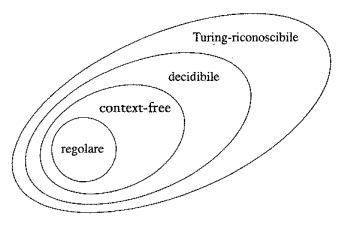
\includegraphics[width=0.45\linewidth]{images/relazioni-classi-linguaggi.png}
    \caption{Relazioni tra le classi di linguaggi}
    \label{fig:relazioni-classi-linguaggi}
\end{figure}

\section{Indecidibilità}
Ora affronteremo il nostro primo teorema che stabilisce l'indecidibilità di uno specifico linguaggio: il problema di determinare se una macchina di Turing accetta una determinata stringa in input. Chiamiamo tale linguaggio $A_{TM}$. Sia
\begin{equation*}
A_{TM} =\{\langle M,w \rangle | M\textit{ è una TM e } M\textit{ accetta }w\}
\end{equation*}

\begin{Thm}{$A_{TM}$ è indecidibile}{}\label{thm:atm-indecidibile}
\textit{$A_{TM}$ è indecidibile.}

\begin{demonstration}
Prima di vedere la dimostrazione, osserviamo che $A_{TM}$ è Turing-riconoscibile. Quindi questo teorema mostra che i riconoscitori sono più potenti dei decisori. La seguente macchina di Turing $U$ riconosce $A_{TM}$.

$U=$ "Su input $\langle M, w\rangle$, dove $M$ è una TM e $w$ è una stringa:
\begin{enumerate}
    \item Simula $M$ su input $w$.
    \item Se durante la computazione $M$ entra nello stato di accettazione, accetta; se $M$ entra nello stato di rifiuto, rifiuta."
\end{enumerate}

Si noti che questa macchina cicla su input $\langle M, w\rangle$ se $M$ cicla su $w$, questo è il motivo per cui non decide $A_{TM}$. Se l'algoritmo avesse modo di determinare che $M$ non si ferma su $w$, sarebbe in tal caso in grado di rifiutare $w$.
\end{demonstration}
\end{Thm}

La macchina di Turing $U$ è, di per sè, interessante. È un esempio del la prima macchina universale di Turing introdotta da Alan Turing nel 1936. Questa macchina è chiamata universale perché è in grado di simulare qualsiasi altra macchina di Turing a partire dalla descrizione di tale macchina.

\subsection{Metodo della diagonalizzazione}
La dimostrazione dell'indecidibilità di $A_{TM}$ utilizza una tecnica chiamata diagonalizzazione.

\begin{Thm}{$\mathcal{R}$ non è numerabile}{}
$\mathcal{R}$ è non numerabile.

\begin{demonstration}
Per dimostrare che $\mathcal{R}$ è non numerabile, mostriamo che non esiste una biezione tra $\mathcal{N}$ e $\mathcal{R}$. La dimostrazione è per assurdo. Supponiamo quindi che esista una biezione $f$ tra $\mathcal{N}$ ed $\mathcal{R}$. Il nostro compito è quello di dimostrare che $f$ non funziona come dovrebbe. Per essere una biezione, $f$ deve associare tutti gli elementi di $\mathcal{N}$ con tutti gli elementi di $\mathcal{R}$. Tuttavia troveremo un numero $X$ in $\mathcal{R}$ che non è accoppiato con alcun elemento in $\mathcal{N}$, il che rappresenterà la contraddizione cercata. Un metodo per trovare questo numero $x$ è quello di costruirlo. Scegliamo ogni cifra di $x$ in modo da renderlo differente da ogni numero reale accoppiato con un elemento di $\mathcal{N}$. Alla fine saremo sicuri che $x$ risulta diverso da ogni numero reale accoppiato con un elemento di $\mathcal{N}$. Possiamo illustrare questa idea con un esempio. Supponiamo che la biezione $f$ esista. Prendiamo $f(1)=3.14159..., f(2)= 55.55555... f(3) ...$ e cosi via. Allora $f$ accoppia il numero 1 con 3.14159..., il numero 2 con 55.55555 e così via.

Costruiamo il numero desiderato, dandone la rappresentazione decimale. Si tratta di un numero compreso tra 0 e 1, quindi tutte le sue cifre significative sono cifre frazionarie che seguono la virgola decimale. Il nostro obiettivo è quello di garantire che $x\neq f(n)$ per ogni $n$. Per garantire $x\neq f(1)$, scegliamo la prima cifra di $x$ come una qualsiasi cifra diversa dalla prima cifra decimale 1 di $f(1) =3.\underline{1}4159...$. Per assicurarci che $x\neq f(2)$ scegliamo la seconda cifra di $x$ diversa dalla seconda cifra decimale 5 di $f(2) =55.5\underline{5}5555...$ Continuando in questo modo lungo la diagonale della tavola per $f$, otteniamo tutte le cifre di $x$. Sappiamo che $x$ non è $f(n)$ per ogni $n$ perché differisce da $f(n)$ nell'$n$-esima cifra frazionaria.
\end{demonstration}
\end{Thm}

\begin{Thm}{Linguaggi non Turing-riconoscibili}{}
\textit{Alcuni linguaggi non sono Turing-riconoscibili.}

\begin{demonstration}
Per dimostrare che l'insieme di tutte le macchine di Turing è numerabile dobbiamo prima osservare che l'insieme di tutte le stringhe $\Sigma^*$ è numerabile, per ogni alfabeto $\Sigma$. Avendo solo un numero finito di stringhe di ogni lunghezza, possiamo formare una lista di $\Sigma^*$ scrivendo tutte le stringhe di lunghezza 0, lunghezza 1, lunghezza 2, e così via. L'insieme di tutte le macchine di Turing è numerabile perché ogni macchina di Turing $M$ può essere codificata con una stringa $\langle M\rangle$. Se ci limitiamo a tralasciare quelle stringhe che non sono la codifica di una macchina di Turing, possiamo ottenere una lista di tutte le macchine di Turing. Per mostrare che l'insieme di tutti i linguaggi è non numerabile, dobbiamo prima osservare che l'insieme delle sequenze binarie infinite è non-numerabile.

Una sequenza binaria infinita è una sequenza senza fine di 0 e 1. Sia $\mathcal{B}$ l'insieme di tutte sequenze binarie infinite. Possiamo dimostrare che $\mathcal{B}$ è non numerabile utilizzando una dimostrazione mediante diagonalizzazione. Sia $\mathcal{L}$ l'insieme di tutti i linguaggi sull'alfabeto $\Sigma$. Mostriamo che $\mathcal{L}$ è non-numerabile dando una corrispondenza con $\mathcal{B}$, dimostrando così che i due insiemi hanno la stessa cardinalità. Sia $\Sigma^* =\{ s_{1}, s_{2}, s_{3} ,...\}$. Ogni linguaggio $A \in \mathcal{L}$ ha un'unica sequenza in $\mathcal{B}$. Il bit $i$-esimo della sequenza è un 1 se $s_{i} \in A$ ed è uno 0 se $s_{i} \notin A$ questa è chiamata la sequenza caratteristica di $A$. Per esempio, se $A$ fosse il linguaggio di tutte le stringhe che iniziano con uno 0 sull'alfabeto $\{0, 1\}$ la sua sequenza caratteristica $\mathcal{X}_{A}$ sarebbe
\begin{gather*}
\Sigma^* = \{\epsilon, 0, 1, 00, 01, 10, 11,000,001,...\}\\
A = \{0, 00, 01,000,001,...\}\\
XA=0\textit{ }1\textit{ }0\textit{ }1\textit{ }1\textit{ }0\textit{ }0\textit{ }1\textit{ }1\textit{ }...
\end{gather*}

La funzione $f:\mathcal{L}\to \mathcal{B}$ dove $f(A)$ è uguale alla sequenza caratteristica di E, è sia iniettiva che suriettiva, quindi è una biezione. Pertanto, essendo $\mathcal{B}$ non numerabile, anche $\mathcal{L}$ è non numerabile.

Abbiamo così dimostrato che l'insieme di tutti i linguaggi non può essere messo in corrispondenza biunivoca con l'insieme di tutte le macchine di Turing. Concludiamo quindi che alcuni linguaggi non sono riconosciuti da una macchina di Turing.   
\end{demonstration}
\end{Thm}

\subsection{Linguaggio indecidibile}
Siamo ora pronti a dimostrare il teorema dell'indecidibilità del linguaggio
\begin{equation*}
A_{TM}=\{\langle M,w\rangle | M\textit{ è una TM ed M accetta }w\}
\end{equation*}

\begin{Thm}{$A_{TM}$ è indecidibile}{}
\textit{$A_{TM}$ è indecidibile.}

\begin{demonstration}
Assumiamo che $A_{TM}$ è decidibile, per poi ottenere una contraddizione. Supponiamo che $H$ sia un decisore per $A_{TM}$. Sull'input $\langle M,w\rangle$, dove $M$ è una TM e $w$ è una stringa, $H$ si ferma ed accetta se $M$ accetta $w$. Inoltre, $H$ si ferma e rifiuta se $M$ non accetta $w$. In altri termini, assumiamo che $H$ è una TM, dove
\begin{equation*}H(\langle M, w\rangle)
\begin{cases}
accetta& \textit{se }M\textit{ accetta }w\\rifiuta& \textit{se }M\textit{ non accetta }w
\end{cases}
\end{equation*}
Ora costruiamo una nuova macchina di Turing $D$ avente $H$ come sottoprocedura. Questa nuova TM chiama $H$ per determinare cosa fa $M$ quando l'input di $M$ è la sua stessa descrizione $\langle M\rangle$. Una volta che $D$ ha determinato questa informazione, essa fa il contrario. Cioè, rifiuta se $M$ accetta ed accetta se $M$ non accetta. Diamo ora una descrizione di $D$.

$D=$ "Su input $\langle M\rangle$, dove $M$ è una TM:
\begin{enumerate}
    \item Esegue $H$ su input $\langle M, \langle M\rangle\rangle$.
    \item Dà in output l'opposto di ciò che $H$ dà in output. Cioè, se $H$ accetta, rifiuta; e se $H$ rifiuta, accetta."
\end{enumerate}
Non lasciatevi confondere dall'idea di attivare una macchina sulla sua stessa descrizione! Ciò è simile all'esecuzione di un programma che chiama se stesso in input, qualcosa che si fa a volte nella pratica. Ricapitolando,
\begin{equation*}D(\langle M\rangle) =
\begin{cases}
accetta& \textit{se }M\textit{ non accetta} \langle M\rangle\\ rifiuta& \textit{se }M\textit{ accetta }\langle M\rangle
\end{cases}
\end{equation*}
Cosa succede quando eseguiamo D con la sua stessa descrizione $\langle D\rangle$ in input? In tal caso, otteniamo
\begin{equation*}D(\langle D\rangle) =
\begin{cases}
accetta& \textit{se }D\textit{ non accetta} \langle D\rangle\\ rifiuta& \textit{se }D\textit{ accetta }\langle D\rangle
\end{cases}
\end{equation*}
Indipendentemente da ciò che $D$ fa, essa è costretta a fare il contrario, il che è ovviamente una contraddizione. Quindi, nè la TM $D$ nè la TM $H$ possono esistere.
\end{demonstration}

La diagonalizzazione diviene evidente quando si esaminano le tavole del comportamento delle TM $H$ e $D$. In queste tavole indicizziamo le righe con tutte le TM $M_{1}, M_{2},...$ e indicizziamo le colonne con le descrizioni $\langle M_{1}\rangle, \langle M_{1}\rangle, ...$ di tali macchine. Le entrate dicono se la macchina di una determinata riga accetta l'input di una data colonna. L'entrata è accetta se la macchina accetta l'input, ma è vuota, se rifiuta o entra in un loop su quell'input.
\begin{center}
\begin{tabular}{|c|c c c c c c c|}
     \hline
     & $\langle M_1\rangle$ & $\langle M_2\rangle$ & $\langle M_3\rangle$ & $\langle M_4\rangle$ & ... & $\langle D\rangle$ & ...\\\hline
     $M_1$ & $\underline{accetta}$ & rifiuta & accetta & rifiuta& & accetta &\\
     $M_2$ & accetta & \underline{accetta} & accetta & accetta& ... & accetta & ...\\
     $M_3$ & rifiuta & rifiuta & \underline{rifiuta} & rifiuta& & rifiuta & \\
     $M_4$ & accetta & accetta & rifiuta &  \underline{rifiuta}& & accetta & \\
     ... & ... & ... & ... & ... & ... & ... & ...\\
     $D$ & rifiuta & rifiuta & accetta & accetta& & \underline{?} & \\
     ... & ... & ... & ... & ... & ... & ... & ...\\\hline
\end{tabular}
\end{center}
\end{Thm}

\subsection{Linguaggio non Turing-riconoscibile}
Il teorema seguente mostra che, se un linguaggio ed il suo complemento sono entrambi Turing-riconoscibili, il linguaggio è decidibile. Quindi, per qualsiasi linguaggio non decidibile, o esso non è Turing-riconoscibile oppure il suo complemento non è Turing-riconoscibile. Ricordiamo che il complemento di un linguaggio è il linguaggio costituito da tutte le stringhe che non sono nel linguaggio. Diciamo che un linguaggio è coTuring-riconoscibile se esso è il complemento di un linguaggio Turing-riconoscibile.

\begin{Thm}{Linguaggio decidibile $\iff$ Turing-riconoscibile e coTuring riconoscibile}{}
\textit{Un linguaggio è decidibile se e solo se è Turing-riconoscibile e coTuring-riconoscibile.}

In altre parole, un linguaggio è decidibile esattamente quando sia esso che il suo complemento sono Turing-riconoscibili.

\begin{demonstration}
Abbiamo due direzioni da dimostrare. In primo luogo, se $A$ è decidibile, possiamo facilmente vedere che sia $A$ che il suo complemento $\overline{A}$ sono Turing-riconoscibili. Qualsiasi linguaggio decidibile è Turing-riconoscibile, e il complemento di un linguaggio decidibile è a sua volta decidibile. Per la direzione inversa, se entrambi $A$ e $\overline{A}$ sono Turing-riconoscibili, indichiamo con $M_{1}$ il riconoscitore per $A$ e con $M_{2}$ il riconoscitore per $\overline{A}$. La seguente macchina di Turing $M$ è un decisore per $A$.

$M =$ "Su input $w$:
\begin{enumerate}
    \item Esegue sia $M_{1}$ che $M_{2}$ su input $w$ in parallelo.
    \item Se $M_{1}$ accetta, accetta; se $M_{2}$ accetta, rifiuta."
\end{enumerate}
L'esecuzione di due macchine in parallelo significa che $M$ ha due nastri, uno per simulare $M_{1}$ e l'altro per simulare $M_{2}$. In questo caso $M$ alterna la simulazione di passo di $M_{1}$ con un passo di $M_{2}$ e continua finché una delle due accetta. Ora dimostriamo che $M$ decide A. Ogni stringa $w$ è in $A$, oppure in $\overline{A}$. Pertanto una tra $M_{1}$ ed $M_{2}$ deve accettare $w$. Poichè $M$ si ferma ogni volta che $M_{1}$ accetta oppure $M_{2}$ accetta, allora $M$ si ferma sempre quindi è un decisore. Inoltre, accetta tutte le stringhe in $A$ e respinge tutte le stringhe che non sono in $A$. Quindi $M$ è un decisore per $A$, e pertanto $A$ è decidibile.
\end{demonstration}
\end{Thm}

\begin{Corollario}{$\overline{A_{TM}}$ non è Turing-riconoscibile}{}
\textit{$\overline{A_{TM}}$ non è Turing-riconoscibile.}

\begin{demonstration}
Sappiamo che $A_{TM}$ è Turing-riconoscibile. Se anche $\overline{A_{TM}}$ fosse Turing-riconoscibile, $A_{TM}$ sarebbe decidibile. Il Teorema \ref{thm:atm-indecidibile} ci dice che $A_{TM}$ non è decidibile, quindi $\overline{A_{TM}}$ non può essere Turing-riconoscibile.    
\end{demonstration}
\end{Corollario}